\usepackage{graphicx}%! Author = Philipp Emmenegger
%! Date = 29/06/2021

\section{Mobile Security}
\subsection{Introduction}
\textbf{Challenges}
\begin{itemize}
    \item Physical security
    \begin{itemize}
        \item Mobile phones can be lost or stolen
        \item Sensitive data on device
        \item Bluetooth, NFC
    \end{itemize}
    \item BYOD - Bring your own device
    \begin{itemize}
        \item Policies
        \item Mobile Device Management
    \end{itemize}
    \item Updates
    \begin{itemize}
        \item Delayed or not available for older / unsupported devices
    \end{itemize}
\end{itemize}

\subsubsection{How to Attack a Smartphone}
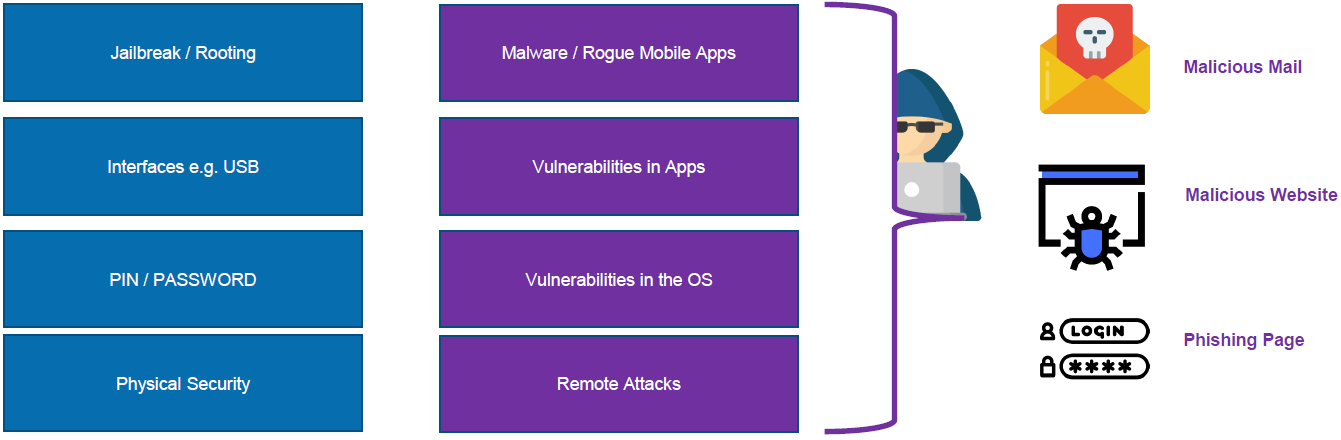
\includegraphics[width=\linewidth]{../img/attack_smartphone.png}

\subsubsection{Mobile Security Threats}
\begin{itemize}
    \item Vulnerabilities in the Mobile Operating System / Bundled Apps
    \item Vulnerabilities in Apps
    \item Untrustworthy devices or software
\end{itemize}

\subsubsection{What malicious actors do}
\textbf{Unique to Smartphones}
\begin{itemize}
    \item Premium SMS messages
    \item Identify location
    \item Record phone calls
    \item Record/Forward/Intercept SMS (2FA)
    \item Encrypt Shared Data = Ransomware
\end{itemize}
\textbf{Similar to Desktop}
\begin{itemize}
    \item Connects to botmasters (DDoS, Crypto-Mining)
    \item Steal data
    \item Phishing
    \item Intercept communication or UI
\end{itemize}

\subsection{Overlay Attacks using Process Scanning}
\begin{itemize}
    \item Malware determines the top most running app
    \item Display a fake screen that is similar to the original app
    \item Used for Automated Transfer Attacks via banking app
\end{itemize}

\subsection{Secure Programming Mobile Apps}
\textbf{Use maximal Security against:}
\begin{itemize}
    \item Lost smartphone
    \item Weak device config (no PIN)
    \item Rouge mobile Apps
    \item Network Man-in-the-Middle
    \item Client Side Code Injection
    \item Insecure Data Storage
    \item App is running on a hacked or untrusted device
\end{itemize}

\subsection{iOS}
\begin{itemize}
    \item Derived from macOS
    \item Unix-like (based on Darwin)
\end{itemize}
\textbf{Common Programming Languages}
\begin{itemize}
    \item Swift
    \item Objective C
    \item C
\end{itemize}
\textbf{Restricted App Distribution}
\begin{itemize}
    \item App Store by Apple
    \item Reviewed by Apple
    \item Code Signing
\end{itemize}
\textbf{Security}
\begin{itemize}
    \item Sandbox Mechanism
    \item File Encryption / Data Protection API
    \item KeyChain
\end{itemize}

\subsubsection{Apple Plattform Security}
\begin{itemize}
    \item Online Documentation
    \item Security by design, integrated into the core
    \item Combination of hardware and software security
    \begin{itemize}
        \item \textbf{Secure Enclave (Processor)}
        \item dedicated co-processor
        \item used for TouchID and KeyChain
    \end{itemize}
\end{itemize}

\subsubsection{iOS Operating System Security}
\textbf{Secure Boot Chain / Root of Trust / Code Signatures}
\begin{itemize}
    \item Prevent execution of third-party / untrusted software
\end{itemize}
\textbf{System Software Authorization}
\begin{itemize}
    \item Prevent downgrade of operating system and firmware
\end{itemize}
\textbf{Secure Enclave / Secure Element}
\begin{itemize}
    \item Isolate crypto operations (Touch / FaceID)
\end{itemize}
\textbf{Lockdown Protocol}
\begin{itemize}
    \item Secures the pairing / communicating with a PC
\end{itemize}
\textbf{File System Encryption / Effaceable Storage}
\begin{itemize}
    \item Prevent unauthorized access to stored data
    \item Secure data deletion
\end{itemize}
\textbf{Sandbox Mechanism / File Data Protection / Keychain}
\begin{itemize}
    \item Application Isolation / Least Privileges
\end{itemize}

\subsubsection{Secure Boot Chain}
\begin{itemize}
    \item Startup in steps
    \item Each step checks integrity of following step: \textbf{Chain of Trust}
    \item Bootrom exploits cannot be patched
\end{itemize}
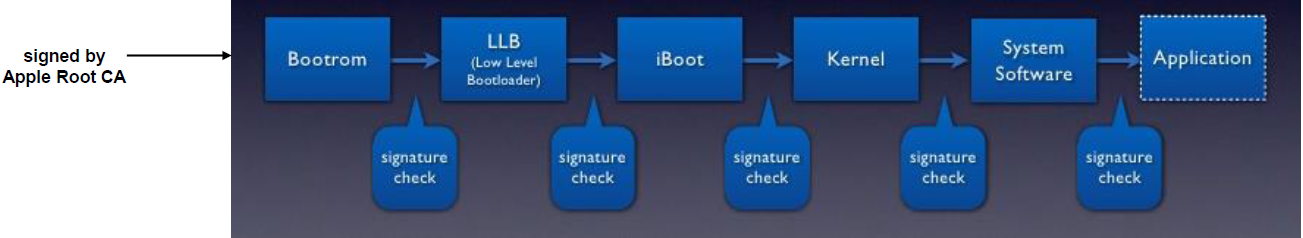
\includegraphics[width=\linewidth]{../img/secure_boot_chain.png}

\subsubsection{App Sandbox}
\begin{itemize}
    \item Each app has its own sandbox
    \item Dedicated directory with subfolders
    \item Isolates data and code
    \item Other apps have no access
    \item Sharing data must be implemented explicitly
    \item Limits damage in case app is compromised
\end{itemize}

\subsubsection{Permission Model}
\begin{itemize}
    \item Permissions are requested when used
    \item Not at installation time
    \item User can deny individually
    \item Can be changed anytime in settings
    \item Usage description since iOS 10
\end{itemize}

\subsubsection{Data Protection API}
\begin{itemize}
    \item \textbf{Every} file is encrypted using AES
    \item Hierarchy of keys
    \item Key handling and en/decryption is part of the secure enclave
    \item Keys are never exposed to the operating system or apps
\end{itemize}
\textbf{Keys:}
\begin{itemize}
    \item Hardware Key: embedded into Crypto component
    \item Passcode Key: derived from Passcode / PIN / Fingerprint
    \item Class Key: encrypted with the above
    \item File Key: encrypted with class key \textbf{unique for each file}
    \item File System Key: protected using hardware key
\end{itemize}
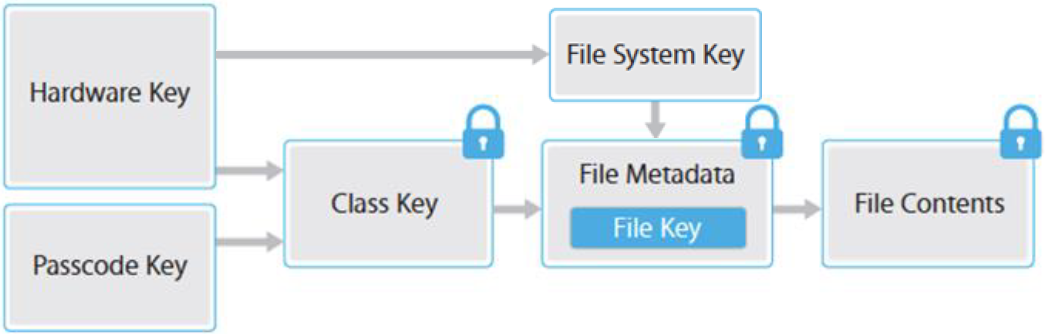
\includegraphics[width=\linewidth]{../img/data_protection_api.png}
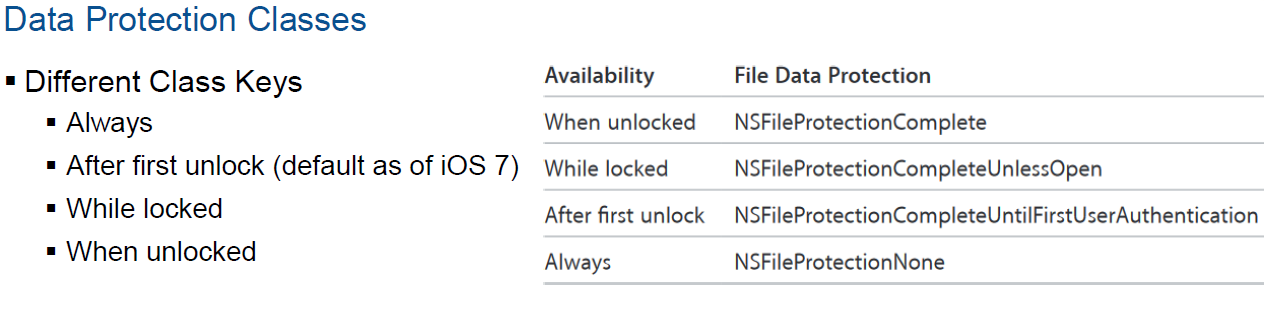
\includegraphics[width=\linewidth]{../img/data_protection_classes.png}

\subsubsection{Keychain API}
\begin{itemize}
    \item SQLite database
    \item Used to store secrets
    \item Keychain respects the sandbox
    \item Protected by hardware
\end{itemize}
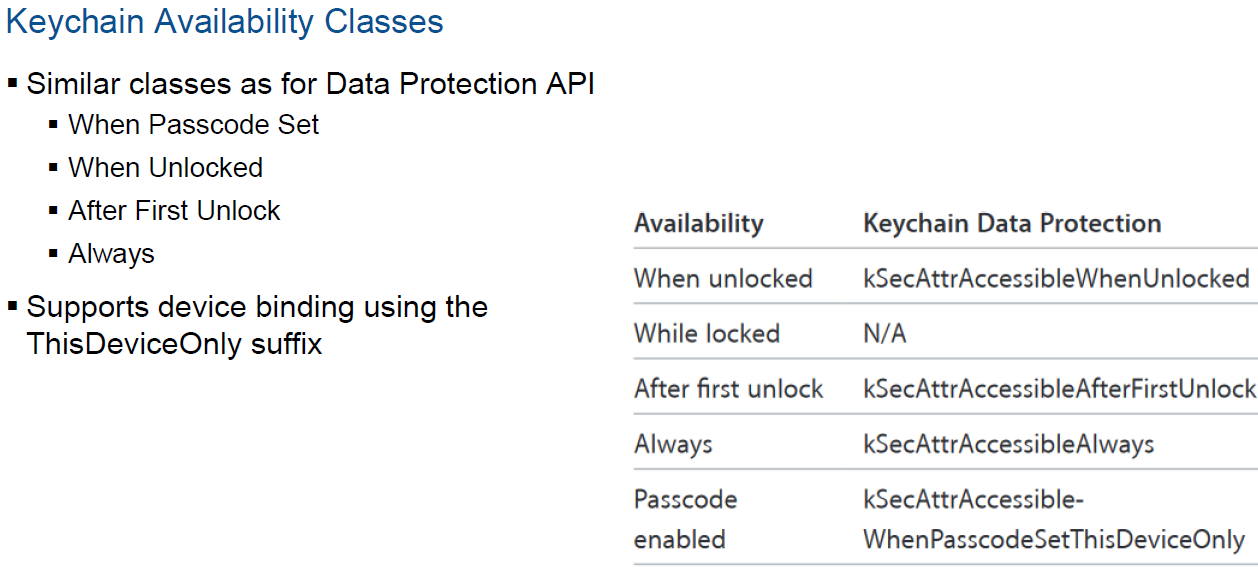
\includegraphics[width=\linewidth]{../img/keychain_classes.png}
\textbf{Keychain Access Control}
\begin{itemize}
    \item Access Control flags define how the item can be accessed
    \item kSecAccessControl, can combine options using and / or
\end{itemize}

\subsubsection{TouchID}
\begin{itemize}
    \item Stored in CPU (Secure enclave)
    \item Not stored server side
\end{itemize}

\subsection{Android}
\textbf{Common Programming Languages}
\begin{itemize}
    \item Kotlin
    \item Java
    \item C
\end{itemize}
\textbf{Restricted App Distribution}
\begin{itemize}
    \item Play store by Google
    \item Alternative stores possible
    \item \textbf{no} review
    \item Coding signing
\end{itemize}
\textbf{Security}
\begin{itemize}
    \item Sandbox Mechanism
    \item File Encryption / Data Protection API
    \item Keychain
\end{itemize}

\subsubsection{App Sandbox}
\begin{itemize}
    \item Each app has own sandbox
    \item Separation using traditional linux permissions
    \item Each app has its own JVM
    \item Isolates data and code - a bit simpler than iOS
    \item Limits damage in case app is compromised
\end{itemize}
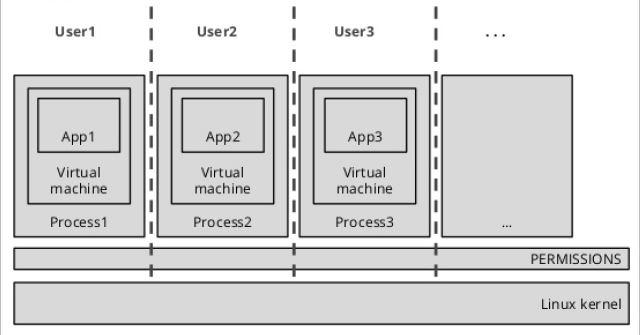
\includegraphics[width=0.6\linewidth]{../img/app_sandbox.png}\\

\subsubsection{Permission Model}
\textbf{Android \textleq 5}
\begin{itemize}
    \item Permissions are requested when installed
    \item take it or leave it
    \item all-or-nothign
\end{itemize}
\textbf{Since Android 6}
\begin{itemize}
    \item Approval at runtime
    \item Can be changed in preferences
\end{itemize}

\subsubsection{Data Encryption}
\begin{itemize}
    \item Full Disk Encryption (FDE)
    \item File Based Encryption (FBE)
\end{itemize}

\subsubsection{Keystore API}
\begin{itemize}
    \item Container for credentials
    \item Can be hardware-backed
\end{itemize}
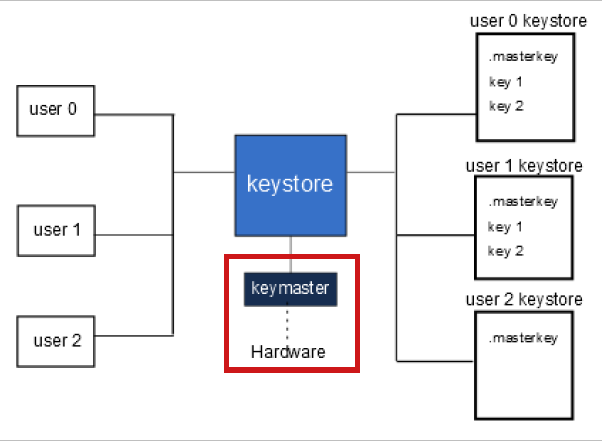
\includegraphics[width=0.6\linewidth]{../img/keystore_api.png}

\subsubsection{Fingerprint API}
\begin{itemize}
    \item Combination with KeyStore
    \item UI in full control of app
\end{itemize}

\subsubsection{Google Play Protect}
\begin{itemize}
    \item Malware scanning
    \item Lost phone tracking / blocking
    \item \textbf{Constantly} scanning apps
\end{itemize}

\subsection{Cross-Plattform \& Hybrid Apps}
\subsubsection{Cross-Plattform Apps}
Often used when trying to reduce software development time by:
\begin{itemize}
    \item Sharing code between multiple platforms
    \item Using established programming languages
    \item Examples:
    \begin{itemize}
        \item Xamarin
        \item React Native
        \item Flutter
    \end{itemize}
\end{itemize}

\subsubsection{Hybrid Apps}
\begin{itemize}
    \item Mobile App development using HTML, JS, CSS
    \item System component renders content
    \begin{itemize}
        \item iOS: WKWebView
        \item Android: WebView
    \end{itemize}
    \item Interactions with native code
\end{itemize}
\textbf{Pros}
\begin{itemize}
    \item Lightweight applications
    \item Portable (write once, use on different plattforms)
    \item Reuse code from web world
\end{itemize}
\textbf{Cons}
\begin{itemize}
    \item Often the UI does not fit the platform's standard
    \item Performance
    \item Security - Same risks as for Web Apps
\end{itemize}

\subsubsection{WebView Hardening}
\begin{itemize}
    \item Proper SSL handling and checking
    \item Implement a white-list for allowed URLS (https only)
    \item Block other protocols
    \item Obfuscate (Javascript) code
    \item Restrict JavaScript and/or file access if possible
\end{itemize}